% vehicle_new Requirements Definition / 要件定義書
% Compile: lualatex requirements.tex

\documentclass[a4paper,11pt]{article}
\usepackage[margin=20mm]{geometry}
\usepackage{tikz}
\usetikzlibrary{positioning, arrows.meta, shapes.geometric, fit, calc}
\usepackage{fontspec}
\usepackage{luatexja-fontspec}
\setmainjfont{Hiragino Kaku Gothic ProN}
\setsansjfont{Hiragino Kaku Gothic ProN}
\setmonofont{Menlo}
\usepackage{booktabs}
\usepackage{enumitem}
\usepackage{xcolor}
\usepackage{fancyhdr}
\usepackage{titlesec}
\usepackage[hidelinks]{hyperref}
\usepackage{listings}

% Colors
\definecolor{accent}{HTML}{2563EB}
\definecolor{accentdark}{HTML}{1E40AF}
\definecolor{subtlegray}{HTML}{6B7280}
\definecolor{lightgray}{HTML}{F3F4F6}
\definecolor{codebg}{HTML}{F8F9FA}
\definecolor{bordercolor}{HTML}{D1D5DB}

% Section styling
\titleformat{\section}
    {\Large\bfseries\color{accentdark}}
    {\thesection.}{0.5em}{}
    [\vspace{-0.5em}\textcolor{bordercolor}{\rule{\textwidth}{0.4pt}}]

\titleformat{\subsection}
    {\large\bfseries\color{accent}}
    {\thesubsection}{0.5em}{}

\titleformat{\subsubsection}
    {\normalsize\bfseries}
    {\thesubsubsection}{0.5em}{}

% Header/Footer
\pagestyle{fancy}
\fancyhf{}
\fancyhead[L]{\small\color{subtlegray}vehicle\_new Requirements Definition}
\fancyhead[R]{\small\color{subtlegray}v0.1 / 2026-04-11}
\fancyfoot[C]{\small\color{subtlegray}\thepage}
\renewcommand{\headrulewidth}{0.4pt}
\renewcommand{\footrulewidth}{0pt}

% Code listing style
\lstset{
    basicstyle=\small\ttfamily,
    backgroundcolor=\color{codebg},
    frame=single,
    rulecolor=\color{bordercolor},
    breaklines=true,
    columns=fullflexible,
}

% Custom table style
\newcommand{\thead}[1]{\textbf{\color{accentdark}#1}}

\begin{document}

% =====================================================================
% Title Page
% =====================================================================
\begin{titlepage}
\begin{center}
\vspace*{40mm}

{\Huge\bfseries\color{accentdark} vehicle\_new}\\[8mm]
{\LARGE Requirements Definition}\\[2mm]
{\LARGE 要件定義書}\\[20mm]

\textcolor{bordercolor}{\rule{0.6\textwidth}{0.4pt}}\\[10mm]

{\large StampFly Ecosystem}\\[2mm]
{\large Next Generation Vehicle Firmware}\\[2mm]
{\large 次世代機体ファームウェア}\\[20mm]

\begin{tabular}{ll}
\color{subtlegray}Version & v0.1 \\
\color{subtlegray}Date & 2026-04-11 \\
\color{subtlegray}Target & ESP32-S3 (M5Stamp S3) + FreeRTOS \\
\color{subtlegray}Platform & 37g Quad-rotor Drone \\
\end{tabular}

\vfill
{\small\color{subtlegray} StampFly Ecosystem Project}
\end{center}
\end{titlepage}

% =====================================================================
% Table of Contents
% =====================================================================
\tableofcontents
\newpage

% =====================================================================
% 1. Purpose
% =====================================================================
\section{目的・方針 / Purpose and Policy}

\subsection{上位目標 / High-Level Goals}

\begin{itemize}[leftmargin=*, itemsep=2pt]
    \item StampFlyの制御ファームウェアとして機能する
    \item 拡張性を持つ
    \item プログラミング教材としてコードの見通しが良い
    \item stampfly\_ecosystemの中核ソフトウェアとしての位置づけを保持する
\end{itemize}

\subsection{直接の動機 / Direct Motivation}

\begin{itemize}[leftmargin=*, itemsep=2pt]
    \item 旧ファームのスパゲッティ化を解消するための再構築
    \item コンポーネント間の責務明確化、状態管理の強化
    \item 意味不明の挙動を設計段階で排除
\end{itemize}

% =====================================================================
% 2. State Model
% =====================================================================
\section{状態モデル / State Model}

\subsection{状態遷移図 / State Transition Diagram}

\begin{center}
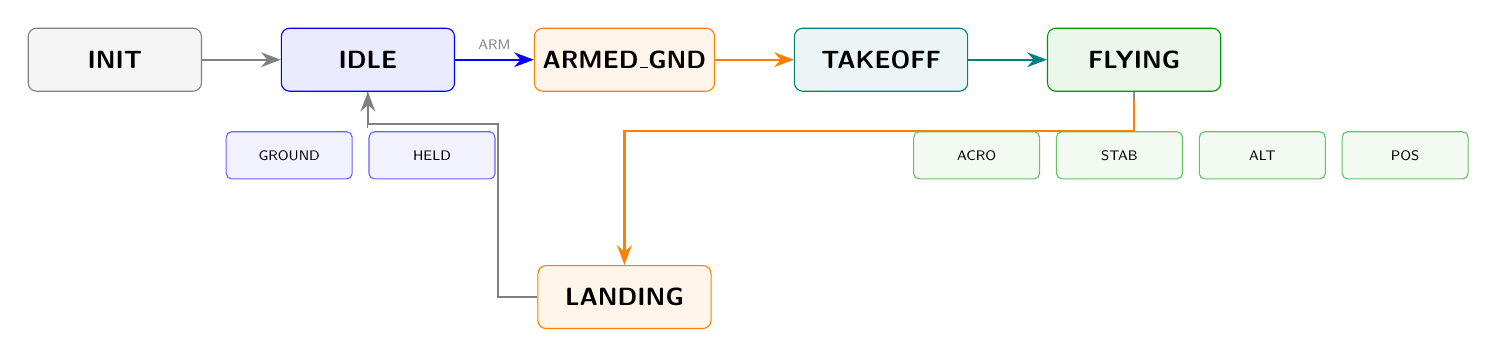
\begin{tikzpicture}[
    every node/.style={font=\sffamily},
    statebox/.style={
        rounded corners=3pt,
        draw=#1,
        fill=#1!8,
        font=\sffamily\small\bfseries,
        minimum width=22mm,
        minimum height=8mm,
        inner sep=3pt,
    },
    subbox/.style={
        rounded corners=2pt,
        draw=#1!60,
        fill=#1!5,
        font=\sffamily\tiny,
        minimum width=16mm,
        minimum height=6mm,
        inner sep=2pt,
    },
    arr/.style={-{Stealth[length=2.5mm]}, thick, #1},
]

\node[statebox=gray] (init) {INIT};
\node[statebox=blue, right=10mm of init] (idle) {IDLE};
\node[statebox=orange, right=10mm of idle] (armed) {ARMED\_GND};
\node[statebox=teal, right=10mm of armed] (takeoff) {TAKEOFF};
\node[statebox=green!60!black, right=10mm of takeoff] (flying) {FLYING};

% Sub-modes under IDLE
\node[subbox=blue, below=5mm of idle, xshift=-10mm] (ground) {GROUND};
\node[subbox=blue, right=2mm of ground] (held) {HELD};

% Sub-modes under FLYING
\node[subbox=green!60!black, below=5mm of flying, xshift=-20mm] (acro) {ACRO};
\node[subbox=green!60!black, right=2mm of acro] (stab) {STAB};
\node[subbox=green!60!black, right=2mm of stab] (alt) {ALT};
\node[subbox=green!60!black, right=2mm of alt] (pos) {POS};

% LANDING
\node[statebox=orange, below=22mm of armed] (landing) {LANDING};

% Arrows - all connections perpendicular to block edges
% Main flow: left to right
\draw[arr=gray] (init.east) -- (idle.west);
\draw[arr=blue] (idle.east) -- node[above, font=\sffamily\tiny, text=gray]{ARM} (armed.west);
\draw[arr=orange] (armed.east) -- (takeoff.west);
\draw[arr=teal] (takeoff.east) -- (flying.west);

% FLYING → LANDING: down from FLYING, then horizontal bar, then down to LANDING.north
\draw[arr=orange] (flying.south) -- ++(0,-5mm) -| (landing.north);

% LANDING → IDLE: left from LANDING, then horizontal, then up to IDLE.south
\draw[arr=gray] (landing.west) -- ++(-5mm,0) -- ++(0,22mm) -| (idle.south);

% Sub-mode indicators
\draw[densely dashed, gray, thin] (idle.south) -- (ground.north -| idle.south);
\draw[densely dashed, gray, thin] (flying.south) -- ++(0,-1mm);

\end{tikzpicture}
\end{center}

\subsection{設計原則 / Design Principles}

\begin{itemize}[leftmargin=*, itemsep=2pt]
    \item ARM/DISARMはアクション（モードではない）
    \item 親状態が共通処理を保証
    \item TAKEOFF/LANDINGは専用モード（離着陸マネージャーが統括）
    \item シーケンス（FLIP, AUTO\_LAND等）は将来拡張可能
    \item FAILSAFEは状態ではなくイベント --- フェイルセーフが \texttt{system.alert} を発行し、状態管理が既存モードへの遷移で対応
\end{itemize}

\subsection{遷移条件 / Transition Conditions}

\begin{table}[h]
\centering
\begin{tabular}{@{}ll@{}}
\toprule
\thead{遷移 / Transition} & \thead{トリガー / Trigger} \\
\midrule
INIT → IDLE\_GROUND & 初期化完了 \\
IDLE\_GROUND ↔ IDLE\_HELD & ToF距離による自動判定 \\
IDLE\_GROUND → ARMED\_GROUND & ARMアクション（ボタン or コントローラ） \\
ARMED\_GROUND → TAKEOFF & スロットル入力 \\
TAKEOFF → FLYING & 離陸完了（高度閾値到達） \\
FLYING内サブモード切替 & コントローラからのモード切替コマンド \\
FLYING → LANDING & パイロット指示 or 自動判定 \\
LANDING → IDLE\_GROUND & 着陸完了 \\
FLYING → ARMED\_GROUND & 静かに着陸 / タッチアンドゴー \\
FLYING → IDLE\_GROUND & 衝突検知 or パイロットDISARM \\
ARMED\_GROUND → IDLE\_GROUND & DISARMアクション \\
\bottomrule
\end{tabular}
\end{table}

% =====================================================================
% 3. Parameter Management
% =====================================================================
\section{パラメータ管理 / Parameter Management}

\begin{table}[h]
\centering
\begin{tabular}{@{}ll@{}}
\toprule
\thead{項目 / Item} & \thead{方針 / Policy} \\
\midrule
固定パラメータ & GPIO、タスク優先度等 → \texttt{constexpr} \\
チューニングパラメータ & PIDゲイン、ESKF設定等 → ランタイム変更可能 \\
命名規則 & 3階層: \texttt{機能.対象.パラメータ} \\
永続化 & NVS \\
追加手順 & 定義 + テーブル登録の2箇所 \\
アクセス手段 & WiFi + CLI \\
コールバック・バリデーション & パラメータ確定後に個別検討 \\
\bottomrule
\end{tabular}
\end{table}

\subsection{命名例 / Naming Examples}

\begin{lstlisting}
rate.roll.kp          # Roll rate proportional gain
rate.roll.ti          # Roll rate integral time
eskf.obs.tof_noise    # ToF observation noise
eskf.process.accel_noise  # Accelerometer process noise
altitude.vel.kp       # Altitude velocity loop Kp
\end{lstlisting}

% =====================================================================
% 4. Components
% =====================================================================
\section{責務分割 / Responsibility Assignment}

14コンポーネントに分割する。

\begin{table}[h]
\centering
\begin{tabular}{@{}cll@{}}
\toprule
\thead{\#} & \thead{コンポーネント / Component} & \thead{責務 / Responsibility} \\
\midrule
1 & センシング / Sensing & センサからデータを読む \\
2 & 状態推定 / State Estimation & 姿勢/位置/速度を推定（差替可能） \\
3 & 状態管理 / State Management & モード遷移、ARM許可判定 \\
4 & フェイルセーフ / Failsafe & 異常検出と対応（状態管理より上位） \\
5 & 離着陸マネージャー / TL Manager & 地上/空中判定、TAKEOFF/LANDING統括 \\
6 & 制御 / Control & セットポイント追従演算（差替可能） \\
7 & アクチュエーション / Actuation & ミキサー＋安全チェック＋モーター出力 \\
8 & コマンド処理 / Command Processing & 全入力ソース吸収・正規化・調停 \\
9 & 通信 / Communication & ESP-NOW/UDP/WiFi送受信 \\
10 & ナビゲーター / Navigator & ウェイポイント、経路計画 \\
11 & キャリブレーション / Calibration & バイアス測定・保存・適用 \\
12 & パラメータ / Parameters & パラメータ保持・変更・永続化 \\
13 & データロガー / Data Logger & Telemetry/Data Stream/Blackbox \\
14 & 通知 / Notification & LED/ブザーで状態表示 \\
\bottomrule
\end{tabular}
\end{table}

\subsection{設計原則 / Design Principles}

\begin{itemize}[leftmargin=*, itemsep=2pt]
    \item 「検出」と「判断」を分離 --- センシングが事実を報告、状態管理が判断する
    \item 制御のインターフェース統一 --- 入力: 推定値+セットポイント、出力: 推力/トルク
    \item 状態推定のインターフェース統一 --- 入力: センサデータ、出力: 姿勢/位置/速度
    \item 状態遷移コールバック（onExit/onEnter）でリセット処理を集約
\end{itemize}

\subsection{コマンド処理の入力ソース / Command Processing Input Sources}

\begin{center}
\begin{tikzpicture}[
    every node/.style={font=\sffamily\small},
    srcbox/.style={rounded corners=2pt, draw=blue!60, fill=blue!5, minimum width=28mm, minimum height=7mm, inner sep=3pt},
    procbox/.style={rounded corners=3pt, draw=accent, fill=accent!8, minimum width=30mm, minimum height=10mm, inner sep=4pt, font=\sffamily\small\bfseries},
    arr/.style={-{Stealth[length=2mm]}, thick, gray},
]

\node[srcbox] (espnow) {ESP-NOW};
\node[srcbox, below=4mm of espnow] (sbus) {SBUS};
\node[srcbox, below=4mm of sbus] (udp) {UDP/WiFi API};
\node[srcbox, below=4mm of udp] (nav) {ナビゲーター};
\node[procbox, right=20mm of sbus, yshift=-2mm] (cmd) {コマンド処理};
\node[right=12mm of cmd, font=\sffamily\small] (sp) {→ セットポイント → 制御};

% Horizontal bar for fork routing
% Each source goes right to a common x, then vertical bar connects to cmd.west
\coordinate (barx) at ([xshift=10mm]espnow.east);

\draw[thick, gray] (espnow.east) -- (barx |- espnow.east);
\draw[thick, gray] (sbus.east) -- (barx |- sbus.east);
\draw[thick, gray] (udp.east) -- (barx |- udp.east);
\draw[thick, gray] (nav.east) -- (barx |- nav.east);

% Vertical bar
\draw[thick, gray] (barx |- espnow.east) -- (barx |- nav.east);

% Junction dots
\fill[gray] (barx |- espnow.east) circle (2pt);
\fill[gray] (barx |- sbus.east) circle (2pt);
\fill[gray] (barx |- udp.east) circle (2pt);
\fill[gray] (barx |- nav.east) circle (2pt);

% Single arrow from bar to cmd
\draw[arr] (barx |- cmd.west) -- (cmd.west);
\fill[gray] (barx |- cmd.west) circle (2pt);

\end{tikzpicture}
\end{center}

% =====================================================================
% 5. Sensors
% =====================================================================
\section{搭載センサ / Sensors}

全センサ搭載（IoT教材として全アクセス可能であることが重要）。

\begin{table}[h]
\centering
\begin{tabular}{@{}lllll@{}}
\toprule
\thead{センサ / Sensor} & \thead{型番 / Part} & \thead{通信 / Bus} & \thead{レート / Rate} & \thead{用途 / Purpose} \\
\midrule
IMU & BMI270 & SPI & 400Hz & 姿勢推定の主センサ \\
地磁気 & BMM150 & I2C & 25Hz & ヨー推定（研究対象） \\
気圧 & BMP280 & I2C & 50Hz & 高度推定（ToF範囲外） \\
ToF（下面） & VL53L3CX & I2C & 30Hz & 高度計測 \\
ToF（前面） & VL53L3CX & I2C & 30Hz & 障害物検知・SLAM \\
OpticalFlow & PMW3901 & SPI & 100Hz & 水平位置推定 \\
電源モニタ & INA3221 & I2C & 10Hz & バッテリー電圧・電流 \\
\bottomrule
\end{tabular}
\end{table}

% =====================================================================
% 6. Actuators
% =====================================================================
\section{搭載アクチュエータ / Actuators}

\begin{table}[h]
\centering
\begin{tabular}{@{}lll@{}}
\toprule
\thead{アクチュエータ / Actuator} & \thead{制御方式 / Control} & \thead{数量 / Qty} \\
\midrule
モーター & LEDC PWM 150kHz 8bit & 4（X-quad配置） \\
ブザー & LEDC PWM トーン生成 & 1 \\
LED（MCU内蔵） & WS2812 RGB & 1 \\
LED（ボード上下） & WS2812 RGB デイジーチェーン & 2 \\
\bottomrule
\end{tabular}
\end{table}

% =====================================================================
% 7. Communication
% =====================================================================
\section{通信 / Communication}

\subsection{機体側の通信 / Vehicle-Side Communication}

\begin{table}[h]
\centering
\begin{tabular}{@{}llll@{}}
\toprule
\thead{名前 / Name} & \thead{目的 / Purpose} & \thead{経路 / Transport} & \thead{初期 / Init} \\
\midrule
Telemetry & モニタリング用（状態表示） & UDP & Yes \\
Data Stream & 解析用（全センサ生値） & UDP / USB（選択） & Yes \\
Blackbox & オンボード記録（クラッシュログ） & 内部Flash（SPIFFS） & Yes \\
CLI & コマンド操作 & USB Serial / TCP & Yes \\
コマンド受信 & RC入力、API & ESP-NOW / UDP & Yes \\
\bottomrule
\end{tabular}
\end{table}

\begin{itemize}[leftmargin=*, itemsep=2pt]
    \item 機体側からWebSocketは撤去（UDP統一、ブロッキングリスク排除）
    \item ブラウザ表示は \texttt{sf monitor web}（UDP→WebSocket変換プロキシ）で対応
    \item スマホ対応は専用アプリ or WebApp
\end{itemize}

\subsection{対応プロトコル / Supported Protocols}

\begin{table}[h]
\centering
\begin{tabular}{@{}ll@{}}
\toprule
\thead{プロトコル / Protocol} & \thead{初期実装 / Initial} \\
\midrule
ESP-NOW（デフォルトRC） & Yes \\
UDP（テレメトリ、制御） & Yes \\
TCP（CLI） & Yes \\
USB Serial（CLI + ログ） & Yes \\
TelloAPI & Yes \\
ROS2 & Yes \\
MAVLink & Yes \\
SBUS（外部RC） & 将来（構造のみ） \\
OTA & しない \\
\bottomrule
\end{tabular}
\end{table}

% =====================================================================
% 8. Timing
% =====================================================================
\section{タイミング要件 / Timing Requirements}

\begin{table}[h]
\centering
\begin{tabular}{@{}lrrl@{}}
\toprule
\thead{タスク / Task} & \thead{周期 / Rate} & \thead{優先度 / Pri} & \thead{スタック / Stack} \\
\midrule
IMU & 400Hz & 24 & 16KB \\
Control & 400Hz（IMU同期） & 23 & 8KB \\
OptFlow & 100Hz & 20 & 8KB \\
Mag & 25Hz & 18 & 8KB \\
Baro & 50Hz & 16 & 8KB \\
Comm & 50Hz & 15 & 4KB \\
ToF & 30Hz & 14 & 8KB \\
Telemetry & 50Hz & 13 & 4KB \\
Power & 10Hz & 12 & 4KB \\
Button & 50Hz & 10 & 4KB \\
LED & 30Hz & 8 & 4KB \\
CLI & 20Hz & 5 & 8KB \\
\bottomrule
\end{tabular}
\end{table}

新責務（フェイルセーフ、離着陸マネージャー等）のタスクマッピングはタスク設計で決定する。

% =====================================================================
% 9. Safety
% =====================================================================
\section{安全要件 / Safety Requirements}

\begin{table}[h]
\centering
\begin{tabular}{@{}lll@{}}
\toprule
\thead{条件 / Condition} & \thead{閾値 / Threshold} & \thead{アクション / Action} \\
\midrule
衝撃（加速度） & 3.0G $\times$ 連続2回 & 自動DISARM \\
異常角速度 & 800 deg/s $\times$ 連続2回 & 自動DISARM \\
通信途絶 & 500ms & ホバリング維持3秒 → 自動着陸 \\
LiPo低電圧 & $\leq$3.4V & ブザー警告のみ \\
USB給電 & $\leq$3.3V & ARM禁止 \\
ESKF発散 & 位置100m or 速度50m/s & ESKFリセット \\
\bottomrule
\end{tabular}
\end{table}

% =====================================================================
% 10. Education
% =====================================================================
\section{教育・拡張性要件 / Education and Extensibility}

\begin{table}[h]
\centering
\begin{tabular}{@{}lll@{}}
\toprule
\thead{項目 / Item} & \thead{方針 / Policy} & \thead{初期 / Init} \\
\midrule
状態推定 & 差替可能（ESKF/EKF/Complementary等） & Yes \\
制御 & 差替可能（PID/MPC/LQR等） & Yes \\
入力ソース & ドライバ追加で拡張 & Yes \\
パラメータ & WiFi変更、NVS永続化 & Yes \\
ナビゲーション & 将来追加可能な構造 & 構造のみ \\
SILシミュレータ & HAL差し替えでPC上動作 & Yes \\
単体テスト & アルゴリズム層をPC上でテスト可能 & Yes \\
コード品質 & 日英バイリンガルコメント、読みやすさ重視 & Yes \\
サンプル集 & 機能別最小動作コード、チュートリアル的コメント & Yes \\
TelloAPI & 標準対応 & Yes \\
ROS2 & 標準対応 & Yes \\
MAVLink & 標準対応 & Yes \\
SBUS & 将来対応 & 構造のみ \\
\bottomrule
\end{tabular}
\end{table}

\end{document}
